\documentclass[titlepage, oneside]{article}
\usepackage{graphicx}
\usepackage{fancyhdr}
\usepackage{url}
\usepackage{sectsty}
\usepackage[margin=1in]{geometry}

\pagestyle{fancy}
\fancyhf{}
\lhead{COMP3005B Project}
\rhead{Edward ``Adam'' Payzant, SN: 101082175}
\sectionfont{\fontsize{12}{15}\selectfont}

\author{Edward ``Adam'' Payzant, SN: 101082175}
\title{COMP3005B Project}

\begin{document}
    \maketitle
    \section{Conceptual Design}
        \subsection{ER Diagram}
            \begin{center}
                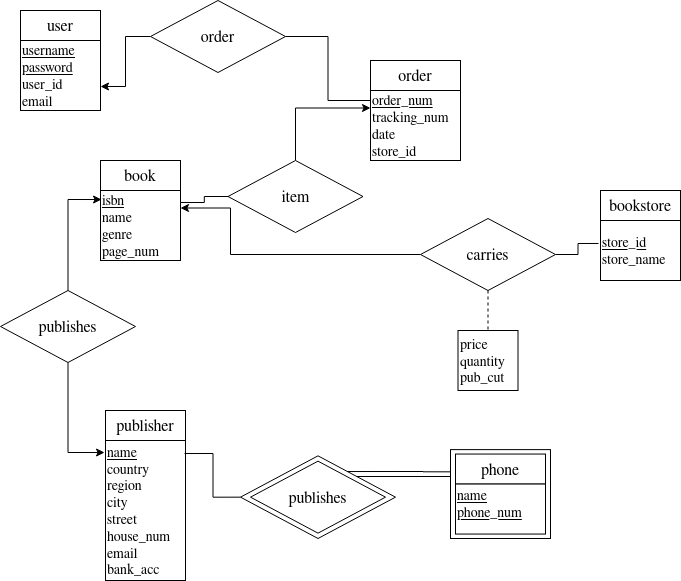
\includegraphics[scale=.65]{images/ERDiagram.png}
                % TODO: FIX "order" relation to "orders"
                % TODO: FIX "publishes" relation to "phone_num"
            \end{center}
        \subsection{Description}
            \begin{itemize}
                \item user: A user account who's only relation is to their orders. Orders can only be linked to one user, but a user can have many orders.
                \item order: Order details. Order items can only link to one order but an order can have many items. Orders can only have one user
                \item book: A book can only have 1 publisher, but can be in muliple orders, carried by multiple bookstores, and be in multiple restocks.
                \item publisher: A publisher can publish multiple books, send multiple restock shipments, and have multiple phones.
                \item phone: phone is a weak entity because it's existence is entirely defined by a publisher. A phone can only tie to one publisher, but a publisher may have multiple phone numbers.
                \item shipment: A shipment can only be sent from one publisher to one bookstore, bute contain multiple books to restock.
                \item bookstore: A bookstore can carry multiple books and receive multiple restock shipments.
            \end{itemize}
        \subsection{Notes}
            \begin{itemize}
                \item The project description states ``When checkingout,  the user inserts billing and shipping information (can be different than those used in registration)''.
                This implies that billing and shipping should be inputted upon registration. I chose not to implement this because it poses an unnecessary security risk for users who have never made an order.
            \end{itemize}
    \section{Reduction to Relation Schema}
        \begin{itemize}
            \item $orders(\underline{user\_id}, \underline{order\_num})$
            \item $item(\underline{order_num}, \underline{isbn})$
            \item $publishes(\underline{isbn}, \underline{publisher})$
            \item $ships(\underline{pub\_name}, \underline{shipment\_id})$
            \item $contains(\underline{isbn}, \underline{shipment\_id}, quantity)$
            \item $receives(\underline{store\_id}, \underline{shipment\_id})$
            \item $carries(\underline{store\_id}, \underline{isbn}, price, quantity, pub\_cut)$
        \end{itemize}
    \section{Normalization of Relation Schema}
    \section{Database Schema Diagram}
        \begin{center}
            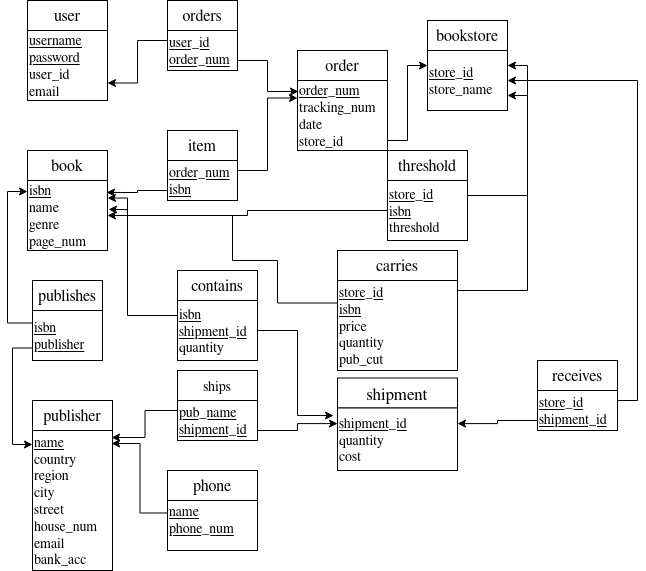
\includegraphics[scale=.6]{images/SchemaDiagram.png}
        \end{center}
    \section{Implementation}
        Implementation is currently incomplete
    \section{Bonus Features}
        \subsection{Implemented Features}
            Currently no bonus features are implemented.
        \subsection{Planned Features}
            \begin{itemize}
                \item Password hashing
                \item HTTPS support
                \item Improved searching
            \end{itemize}
    \section{GitHub Repo}
        Repository will be made public April 15. \\
        \url{https://github.com/AdamPayzant/COMP3005_Project}
\end{document}